\documentclass{article}
\usepackage[top=1in,bottom=1in]{geometry}
\usepackage{hyperref}
\usepackage{amsmath}
\usepackage{amssymb}
\usepackage{graphicx}
\usepackage{tikz}
\usetikzlibrary{automata}
\usetikzlibrary{positioning}
\usetikzlibrary{arrows}
\tikzset{node distance=2.5cm, % Minimum distance between two nodes. Change if necessary.
every state/.style={ % Sets the properties for each state
semithick,
fill=gray!10},
initial text={}, % No label on start arrow
double distance=2pt, % Adjust appearance of accept states
every edge/.style={ % Sets the properties for each transition
draw,
->,>=stealth', % Makes edges directed with bold arrowheads
auto,
semithick}}
\setlength{\parindent}{0pt}
\graphicspath{ {./assets/} }
\usepackage[none]{hyphenat}
\date{}
\title{CMSC452 Elementary Theory of Computation}
\begin{document} 
  \author{Michael Li}
  \title{CMSC452 Elementary Theory of Computation}
  \maketitle
  \tableofcontents
  \newpage
  \section{DFA $(Q, \Sigma, \delta, s, F)$}
  \textbf{Modulo}: $L = \{w \colon \#_a(w) \equiv 3 \pmod 5\}$

  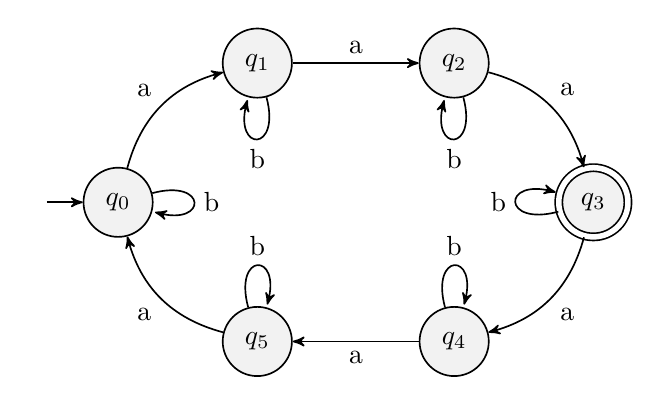
\begin{tikzpicture}
    \node[state, initial] (q0) {$q_0$};
    \node[state, above right of=q0] (q1) {$q_1$};
    \node[state, right of=q1] (q2) {$q_2$};
    \node[state, below right of=q2, accepting] (q3) {$q_3$};
    \node[state, below left of=q3] (q4) {$q_4$};
    \node[state, left of=q4] (q5) {$q_5$};
    \draw (q0) edge[bend left] node {a} (q1);
    \draw (q0) edge[loop right] node {b} (q0);
    \draw (q1) edge node {a} (q2);
    \draw (q1) edge[loop below] node {b} (q1);
    \draw (q2) edge[bend left] node {a} (q3);
    \draw (q2) edge[loop below] node {b} (q2);
    \draw (q3) edge[bend left] node {a} (q4);
    \draw (q3) edge[loop left] node {b} (q3);
    \draw (q4) edge node {a} (q5);
    \draw (q4) edge[loop above] node {b} (q4);
    \draw (q5) edge[bend left] node {a} (q0);
    \draw (q5) edge[loop above] node {b} (q5);
  \end{tikzpicture}
  \bigskip

  \textbf{Intersection}: $L = \{w \colon \#_a(w) \equiv 3 \pmod 5 \wedge \#_b(w) \equiv 2 \pmod 3\}$

  $Q = \{0, \ldots, 4\} \times \{0, \ldots, 2\}$

  $\Sigma = \Sigma$

  $\delta((q_1, q_2), \sigma) = (\delta_1(q_1, \sigma), \delta_2(q_2, \sigma))$

  $s = (0, 0)$

  $F = F_1 \times F_2$
  \bigskip

  \textbf{Expanded Notation}: Number written in base 10 with mod 7

  $10^0 \pmod 7 = 1$

  $10^1 \pmod 7 = 3$

  $10^2 \pmod 7 = 2$

  $10^3 \pmod 7 = 6$

  $10^4 \pmod 7 = 4$

  $10^5 \pmod 7 = 5$

  $10^6 \pmod 7 = 1$
  \medskip

  $Q = \{0, \ldots, 6\} \times \{0, \ldots, 5\}$ Keep track of weighted sum $\pmod 7$ and track digit placement $\pmod 6$

  $\Sigma = \{0, \ldots, 9\}$

  $\delta(a, 0), i) = (a + 1*i \pmod 7, 1)$

  $\delta(a, 1), i) = (a + 3*i \pmod 7, 2)$

  $\delta(a, 2), i) = (a + 2*i \pmod 7, 3)$

  $\delta(a, 3), i) = (a + 6*i \pmod 7, 4)$

  $\delta(a, 4), i) = (a + 4*i \pmod 7, 5)$

  $\delta(a, 5), i) = (a + 5*i \pmod 7, 0)$

  $s = (0, 0)$

  \bigskip

  \textbf{Minimum Number of DFA States Proof}: $a^n$ requires $n$ states

  By pigeonhole principle, if a DFA requires $n-1$ states, 2 of the states, $q_i, q_j$ ($i \neq j$), must be the same.  Then
  \[a^ia^{n-i} = a^n \neq a^ja^{n-i}\]
  Thus contradiction is reached and DFA requires at least $n$ states.\bigskip

  \textbf{DFA Complementation}: $L(Q, \Sigma, \delta, s, Q - F)$ \bigskip

  \textbf{DFA Capabilities}
  \begin{itemize}
    \item DFA can track $#_a(w) \pmod{17}$
    \item DFA cannot track $#_a(w)$
    \item If DFA $M$ exists and $L(M) = L$, then $L$ is regular
  \end{itemize}
    \section{NFA $(Q, \Sigma, \Delta, s, F)$}
    \textbf{Important}: $\Delta \colon Q \times (\Sigma \cup \{e\}) \rightarrow 2^{Q}$ is a set of possible resultant states \bigskip

    \textbf{Union}: $L = \{w \colon \#_a \equiv 0 \pmod 3 \vee w \colon \#_b \equiv 0 \pmod 4\}$

  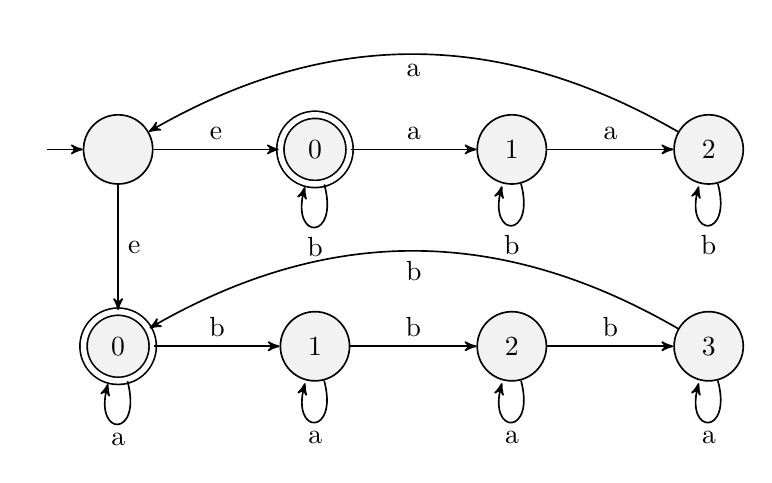
\begin{tikzpicture}
    \node[state, initial] (q0) {};
    \node[state, accepting, right of=q0] (q1) {0};
    \node[state, right of=q1] (q2) {1};
    \node[state, right of=q2] (q3) {2};
    \node[state, below of=q0, accepting] (q4) {0};
    \node[state, right of=q4] (q5) {1};
    \node[state, right of=q5] (q6) {2};
    \node[state, right of=q6] (q7) {3};
    \draw (q0) edge node {e} (q1);
    \draw (q1) edge node {a} (q2);
    \draw (q1) edge[loop below] node {b} (q1);
    \draw (q2) edge node {a} (q3);
    \draw (q2) edge[loop below] node {b} (q2);
    \draw (q3) edge[bend right] node {a} (q0);
    \draw (q3) edge[loop below] node {b} (q3);
    \draw (q0) edge node {e} (q4);
    \draw (q4) edge[loop below] node {a} (q4);
    \draw (q4) edge node {b} (q5);
    \draw (q5) edge[loop below] node {a} (q5);
    \draw (q5) edge node {b} (q6);
    \draw (q6) edge[loop below] node {a} (q6);
    \draw (q6) edge node {b} (q7);
    \draw (q7) edge[bend right] node {b} (q4);
    \draw (q7) edge[loop below] node {a} (q7);
  \end{tikzpicture}
  \bigskip

  \textbf{Not Equivalent Modulo}: $a^n \colon n \not\equiv 0 \pmod{15}$ 

  Equivalent of $L = \{w \colon \#_a \not\equiv 0 \pmod 3 \vee w \colon \#_a \not\equiv 0 \pmod 5\}$ \bigskip

  \textbf{Equivalent Modulo}: $a^n \colon n \equiv 0 \pmod{15}$ 

  This requires $15$ states. Proof using pigeon hole principle. \bigskip

  \textbf{Converting NFA to DFA}: result DFA will have $\leq 2^n$ states
  \begin{enumerate}
    \item Remove $e$-transitions and create a new transition function $\Delta_1$

    \[\Delta_1(q, \sigma) = \bigcup_{0 \leq i, j \leq n} \Delta(q, e^i\sigma e^j)\]
    \item Define DFA that recognizes NFA $M(Q, \Sigma, \Delta_1, s, F)$

      DFA $(2^Q, \Sigma, \delta, \{s\}, F')$ will keep track of the \textbf{set of states} the NFA could be in

      $\delta \colon 2^Q \times \Sigma = 2^Q$

      $\delta(A, \sigma) = \bigcup\limits_{q \in A} \Delta_1(q, \sigma)$

      $F' = \{A \colon A \cap F \neq \emptyset\}$
  \end{enumerate}

  \textbf{Complement}:

    Complement with NFA is difficult because we can't flip normal/final states. Instead we have to
    \begin{enumerate}
      \item Convert $n$-NFA to $2^n$-DFA
      \item Take complement of DFA $\implies 2^n$-DFA
      \item So we have a $2^n$ NFA
    \end{enumerate}
  \textbf{NFA Capabilities}:
  \begin{itemize}
    \item If NFA $M$ exists and $L(M) = L$, then $L$ is regular
  \end{itemize}
  \section{Regex}
  \begin{enumerate}
    \item Base Case: contains $e$ and $\sigma \in \Sigma$
    \item If $\alpha$ and $\beta$ are regular, then $\alpha \cup \beta$ and $\alpha \beta$ are regular
    \item $\alpha$ is regular then $\alpha^*$ is regular
  \end{enumerate}
  $L(\alpha)$ is the set of strings generate from a regex $\alpha$\bigskip

  \textbf{Proof Regex $\subseteq$ NFA}

  Base Case: $e$ and $\{\sigma\}$ have NFAs

  IH: Assume for every regex $\beta$ with $|\beta|$ < $n$, $L(\beta)$ is recognized by an NFA

  IS: Show $\alpha$ is a regex, with $|\alpha| = n$
  \begin{itemize}
    \item Case 1: $\alpha = \alpha_1 \cup \alpha_2$. Since $|\alpha_1|, |\alpha_2 < n$, we can apply IH and generate NFAs $N_1$ and $N_2$ such that $L(N_1) \cup L(N_2) = L(\alpha)$
    \item Case 2: similar for $\alpha = \alpha_1 \circ \alpha_2$
    \item Case 3: similar for $\alpha = \alpha_1^*$
  \end{itemize}
  Thus, regex $\subseteq$ NFA $\subseteq$ DFA \bigskip

  \textbf{Proof DFA $\subseteq$ Regex}

  For the sake of the proof, we can extend $\delta \colon Q \times \Sigma^* \rightarrow Q$ to handle strings

  so $\delta(q, w = $ state we end up at if we start at $q$ and input $w$ \medskip

  Key idea is for every pair of states $(i,j)$, we find the regex that represents the string that takes from state $i$ to state $j$

  $R(i, j, k) = \{w \colon \delta(i, w) = j \text{ using only states } \{1, \ldots, k\} \}$ \medskip

  Base case: $R(i, j, 0)$ for $1 \leq i,j \leq n$. Strings with no intermediary state so a single transition or $i = j$ and string is $e$
  \[R(i, j, 0) = 
    \begin{cases}
    \{\sigma \colon \delta(i, \sigma) = j\} & i \neq j\\
    \{\sigma \colon \delta(i, \sigma) = j\} \cup \{e\} & i = j\\
  \end{cases}
  \]
  IH: Assume for $1 \leq i, j \leq n$, $R(i, j, k-1)$ is a regex

  IS: Prove for all $1 \leq i, j \leq n$, $R(i, j, k)$ is a regex
  \[R(i, j, k) = R(i, j, k-1) \cup R(i, k, k-1)\circ R(k, k, k-1)^* \circ R(k,j, k-1)\]
  \textbf{Capabilities of Regex}
  \begin{itemize}
    \item Regex can't cleanly represent complement, although it is regular: idea is to convert $n$-NFA to $2^n$-DFA, take the complement, then convert to a $2^{2^n}$ regex
    \item Regex can't cleanly represent intersection, although it is regular: idea is to convert to an NFA then convert back to regex
  \end{itemize}
  \subsection{Trex}
  \begin{enumerate}
    \item Base Case: contains $e$ and $\sigma \in \Sigma$
    \item If $\alpha$ and $\beta$ are regular, then $\alpha \cup \beta$ and $\alpha \beta$ are regular
    \item $\alpha$ is regular then $\alpha^*$ is regular
    \item If $\alpha$ is a trex and $n \in \mathbb{N}$ then $\alpha^n$ takes $O(\lg{n})$ space
  \end{enumerate}
  \section{Number of States}


  \textbf{Small NFA}: $L = \{a^i \colon i \neq 500\}$
    \begin{itemize}
      \item For $i \geq 501$, use

        \textbf{Frobenius Theorem}: for all $ z \geq xy - x - y + 1$ there is $c, d \in \mathbb{N}$ such that $z = cx + cy$

        For all $z \geq 500 = 51*11 - 51 - 11 + 1$, there is a $c,d \in \mathbb{N}$ such that $z = cx = cy$

        Thus, $ z + 1 \geq 501 = 51 * 11 - 51 - 11 + 2$ and we create an NFA for this
      \item For $i \leq 499$, use the following property of coprimes:

        Let $\{q_1, \ldots, q_k\}$ be a set of coprimes such that $\prod_{i = 1}^{k}q_i \geq n$

        Then the set of $i$ such that:

        $i \not\equiv n \pmod{q_1}$

        $\ldots$

        $i \not\equiv n \pmod{q_k}$
        
        Contains $\{1, \ldots, n -1 \}$ but does not contain $n$

        This will take $O((\log{n})^2\log{\log{n}})$ to represent using NFAs

      \begin{tikzpicture}[shorten >=1pt,node distance=1.8cm,on grid,auto] 
         \node[state] (q_0)   {}; 
         \node[state] (a_0) [right=of q_0] {0}; 
         \node[state, accepting] (a_1) [above right=of a_0] {1}; 
         \node[state] (a_2) [above right=of a_1] {2}; 
         \node[state] (a_n) [below right=of a_2] {$\ldots$}; 
         \node[state] (a_50) [below right=of a_0] {50}; 
         \node[state] (a_49) [below right=of a_50] {49}; 
         \node[state] (a_m) [below right=of a_49] {$\ldots$}; 
         \node[state] (a_41) [right=of a_m] {$41$}; 
         \node[state, accepting] (b_0) [above=of q_0] {}; 
         \node[state, accepting] (b_1) [above left=of b_0] {}; 
         \node[state, accepting] (b_2) [above=of b_1] {}; 
         \node[state] (b_3) [above right=of b_2] {3}; 
         \node[state, accepting] (b_4) [right=of b_3] {}; 
         \node[state, accepting] (b_5) [below right=of b_4] {}; 
         \node[state, accepting] (b_6) [below=of b_5] {}; 
         \node[state, accepting] (c_0) [below=of q_0] {}; 
         \node[state, accepting] (c_1) [below left=of c_0] {}; 
         \node[state, accepting] (c_2) [below=of c_1] {}; 
         \node[state, accepting] (c_3) [below right=of c_2] {}; 
         \node[state] (c_4) [below right=of c_3] {4}; 
         \node[state, accepting] (c_5) [above right=of c_4] {}; 
         \node[state, accepting] (c_6) [above=of c_5] {}; 
         \node[state, accepting] (c_7) [above left=of c_6] {}; 
         \node[state, accepting] (d_0) [left=of q_0] {}; 
         \node[state, accepting] (d_1) [below left=of d_0] {}; 
         \node[state, accepting] (d_2) [below left=of d_1] {}; 
         \node[state, accepting] (d_3) [left=of d_2] {}; 
         \node[state, accepting] (d_4) [above=of d_3] {}; 
         \node[state] (d_5) [above=of d_4] {5}; 
         \node[state, accepting] (d_6) [above right=of d_5] {}; 
         \node[state, accepting] (d_7) [above right=of d_6] {}; 
         \node[state, accepting] (d_8) [below right=of d_7] {}; 
          \path[->] 
          (q_0) edge  node {$\epsilon$} (a_0)
          (q_0) edge  node {$\epsilon$} (b_0)
          (q_0) edge  node {$\epsilon$} (c_0)
          (q_0) edge  node {$\epsilon$} (d_0)
          (a_0) edge[bend left=5]  node {$a$} (a_1)
          (a_1) edge[bend left=5]  node {$a$} (a_2)
                edge  node {$e$} (a_41)
          (a_2) edge[bend left=5]  node {$a$} (a_n)
          (a_n) edge[bend left=5]  node {$a$} (a_41)
          (a_41) edge[bend left=5]  node {$a$} (a_m)
          (a_m) edge[bend left=5]  node {$a$} (a_49)
          (a_49) edge[bend left=5]  node {$a$} (a_50)
          (a_50) edge[bend left=5]  node {$a$} (a_0)
          (b_0) edge[bend left=5]  node {$a$} (b_1)
          (b_1) edge[bend left=5] node {$a$} (b_2)
          (b_2) edge[bend left=5] node {$a$} (b_3)
          (b_3) edge[bend left=5] node {$a$} (b_4)
          (b_4) edge[bend left=5] node {$a$} (b_5)
          (b_5) edge[bend left=5] node {$a$} (b_6)
          (b_6) edge[bend left=5] node {$a$} (b_0)
          (c_0) edge node {$a$} (c_1)
          (c_1) edge node {$a$} (c_2)
          (c_2) edge node {$a$} (c_3)
          (c_3) edge node {$a$} (c_4)
          (c_4) edge node {$a$} (c_5)
          (c_5) edge node {$a$} (c_6)
          (c_6) edge node {$a$} (c_7)
          (c_7) edge node {$a$} (c_0)
          (d_0) edge[bend left=5] node {$a$} (d_1)
          (d_1) edge[bend left=5] node {$a$} (d_2)
          (d_2) edge[bend left=5] node {$a$} (d_3)
          (d_3) edge[bend left=5] node {$a$} (d_4)
          (d_4) edge[bend left=5] node {$a$} (d_5)
          (d_5) edge[bend left=5] node {$a$} (d_6)
          (d_6) edge[bend left=5] node {$a$} (d_7)
          (d_7) edge[bend left=5] node {$a$} (d_8)
          (d_8) edge[bend left=5] node {$a$} (d_0)
      \end{tikzpicture}
      Above, $\pmod 7$. Below $\pmod 8$. Left $\pmod 9$

    \end{itemize}

    \bigskip
  \textbf{Proof $\Sigma^*a\Sigma^n$ Requires $2^{n+1}$ DFA States}
    
  \bigskip

  \textbf{Number of States DFA/NFA/Regex}: \medskip

   \begin{tabular}{||c c c c||} 
     \hline
     Closure Property & DFA & NFA & Regex\\ [0.5ex] 
     \hline
     $L_1 \cup L_2$ & $n_1n_2$ & $n_1 + n_2 + 1$ & $L_1 + L_2$\\
     $L_1 \cap L_2$ & $n_1n_2$ & $n_1n_2$ & $X$\\
     $L_1 \circ L_2$ & $X$ & $n_1 + n_2$ & $L_1 + L_2$\\
     $\overline{L}$ & $n$ & $X$ & $X$\\
     $L^*$ & $X$ & $n + 1$ & $L + 1$\\
     \hline
    \end{tabular}
  \section{Pumping Lemma}
  If $L$ is regular then there exists $n_0, n_1$ such that for all $w \in L$ where $|w| \geq n_0$, there exists an $x, y, z$ such that
  \begin{itemize}
    \item $w = xyz$ and $y \neq e$
    \item $|xy| \leq n_1$ (aka $xy$ is short)
    \item for all $i \geq 0$, $xy^iz \in L$
  \end{itemize}
  To prove $L$ is not regular need to find some $i$ such that $xy^iz \not\in L$ \bigskip

  \textbf{Example}: $L = \{a^nb^n \colon n \in \mathbb{N}\}$ not regular

  Let $xy$ contain only $a$'s so

  $x = a^{m_1}$

  $y = a^{m_2}$

  $z = a^{n-m_1-m_2}b^n$

  Take $i = 2$ then
  \[a^{m_1 + 2m_2 + n - m_1 - m_2}b^n = a^{n + m_1}b^{n}\] 
   which is clearly not in L\bigskip

  \textbf{Example}: $L = \{w \colon \#_a(w) \neq \#_b(w)\}$ not regular

  Pumping Lemma doesn't work b/c there's not way of controlling the number of $a$ output

  However we know that $L_2= \{w \colon \#_a(w) = \#_b(w)\}$ is not regular so we can take the complement of $L_2$, which will be not regular. \bigskip

  \textbf{Example}: $L = \{a^{n^2} \colon n \in \mathbb{N}\}$  not regular
  Let $x = a^{n_1}$, $y = a^{n_2}$, and $z = a^{n_3}$ so

  \[a^{n_1}(a^{n_2})^ia^{n_3} \in L\]
  So $\forall i \geq 0, n_1 + in_2 + n_3$ is a square

  $(n_1 + n_3) = x^2$

  $(n_1 + n_3) + n_2 \geq (x+1)^2$

  $\ldots$

  $(n_1 + n_3) + n_i \geq x^2 + 2ix + i^2 \implies \frac{(n_1 + n_3)}{i} + n_2 \geq i$ so LHS decreases while RHS grows so this can't hold for all $i$ \bigskip

  \textbf{Example}: $L = \{a^nb^m \colon n > m\}$ not regular

  Revise pumping lemma to bound $|yz|$ then do pumping on the $b$'s \bigskip

  \textbf{Example}: $L = \{a^{n_1}b^mc^{n_2}\}$ not regular

  Let $w = a^n b^{n-1} c^n$ and $x = a^{n_1}, y = a^{n_2} z = a^{n - n_1 - n_2}b^{n-1}c^n$. Take $i = 0$. Then

  \[xy^0z = a^{n-n_1}b^{n-1}c^n\]
  $\#_a$ on the left side is clearly $\leq$ than $\#_b$, which is $(n-1)$. Thus $xy^0z \not\in L$.
  \section{CFG (N, \Sigma, R, S)}
  \textbf{Not CFL Examples}
  \begin{itemize}
    \item $\{a^n b^n c^n\}$
    \item $\{a^{n^2}\}$
    \item If $L \subseteq a^*$ and $L$ is not regular, then $L$ is not context free
    \item $L_1 \cap L_2$
    \item $\overline{L}$
  \end{itemize}

  \textbf{Proof Regex $\subseteq$ CFG}

  Base case $|\alpha| = 1$ then $\sigma$ or $e$ are both CFL's

  IH: For regex $\beta$ with $|\beta| < n$ there exists a CFG $G$ such that $L(\beta) = L(G)$

  IS: Take a regex $\alpha$ with $|\alpha| = n$

  Case 1: $\alpha = \beta_1 \cup \beta_2$. By IH, $\beta_1$ and $\beta_2$ are CFL, and by closure under $\cup$, $L(\alpha)$ is a CFL
  
  Case 2: Similar closure for $\alpha = \beta_1 \circ \beta_2$

  Case 3: Similar closure for $\alpha = \beta^*$ \bigskip

  \textbf{Chomsky Normal Form}

  \begin{enumerate}
    \item $A \rightarrow BC$ where $A,B,C \in N$
    \item $A \rightarrow \sigma$ where $A \in N, \sigma \in \Sigma$
    \item $S \rightarrow e$ where $S$ is the start state
  \end{enumerate}

  \textbf{Difference between DFA, NFA, CFG Sizes}: $L = \{a, b\}^* a \{a, b\}^n$

  DFA requires $\Theta(2^n)$

  NFA requires $n + \Theta(1)$

  CFG requires $\Theta(\lg(n))$

  CFG can be constructed by having $L = L_1 \circ L_2$ where
  \begin{itemize}
    \item $L_1 = \{a, b\}^*a$ which requires 5 rules:

      $A \rightarrow AS$
      
      $S \rightarrow BS$

      $S \rightarrow a$

      $A \rightarrow a$

      $B \rightarrow b$

    \item $L_2 = \{a,b\}^n$ which can be constructed in $\lg(n)$ rules assuming $n$ is a power of $2$:

      $S \rightarrow S_1S_2$

      $S_1 \rightarrow S_2S_2$

      $\ldots$

      $S_{\lg(n)} \rightarrow a$

      $S_{\lg(n)} \rightarrow b$
  \end{itemize}
\end{document}
